\chapter{Esecuzione}
\label{ch:results}
Qui vengono confrontati i due algoritmi REPTree e RIPPER/JRip. Entrambi hanno sfruttato una \textit{10-fold cross validation}.

\section{Risultati su \texttt{German Credit}}

\normalsize L'esecuzione ha coinvolto 900 istanze di training e 100 istanze di testing ad ogni iterazione del CV.

\begin{mdframed}[frametitle=Esecuzione NaiveBayesSimple]
	\footnotesize\verbatiminput{results/nb/german_credit.nb}
\end{mdframed}

\LTXtable{1.4\linewidth}{results/nb/german_credit.nbc}


\begin{mdframed}[frametitle=Esecuzione REPTree]
	\footnotesize\verbatiminput{results/reptree/german_credit.reptree}
\end{mdframed}


\begin{sidewaysfigure}
	\thisfloatpagestyle{empty}
	\makebox[\textwidth]{
\includegraphics[width=1.4\textwidth, height=.4\textheight]{results/reptree/gc.pdf}}
	\caption{Modello di REPTree}
\end{sidewaysfigure}

\pagebreak

\begin{mdframed}[frametitle=Esecuzione JRip]
	\footnotesize\verbatiminput{results/jrip/german_credit.jrip}
\end{mdframed}


\noindent
\normalsize Regole:
\input{results/jrip/german_credit.list.rules}

\pagebreak

\section{Risultati su \texttt{Hepatitis}}

\normalsize L'esecuzione ha coinvolto 139 istanze di training e 16 istanze di testing ad ogni iterazione del CV.

\begin{mdframed}[frametitle=Esecuzione NaiveBayesSimple]
	\footnotesize\verbatiminput{results/nb/hepatitis.nb}
\end{mdframed}


\scriptsize\input{results/nb/hepatitis.nbc}

\begin{mdframed}[frametitle=Esecuzione REPTree]
	\footnotesize\verbatiminput{results/reptree/hepatitis.reptree}
\end{mdframed}


\begin{figure}[htb]
	\makebox[\textwidth]{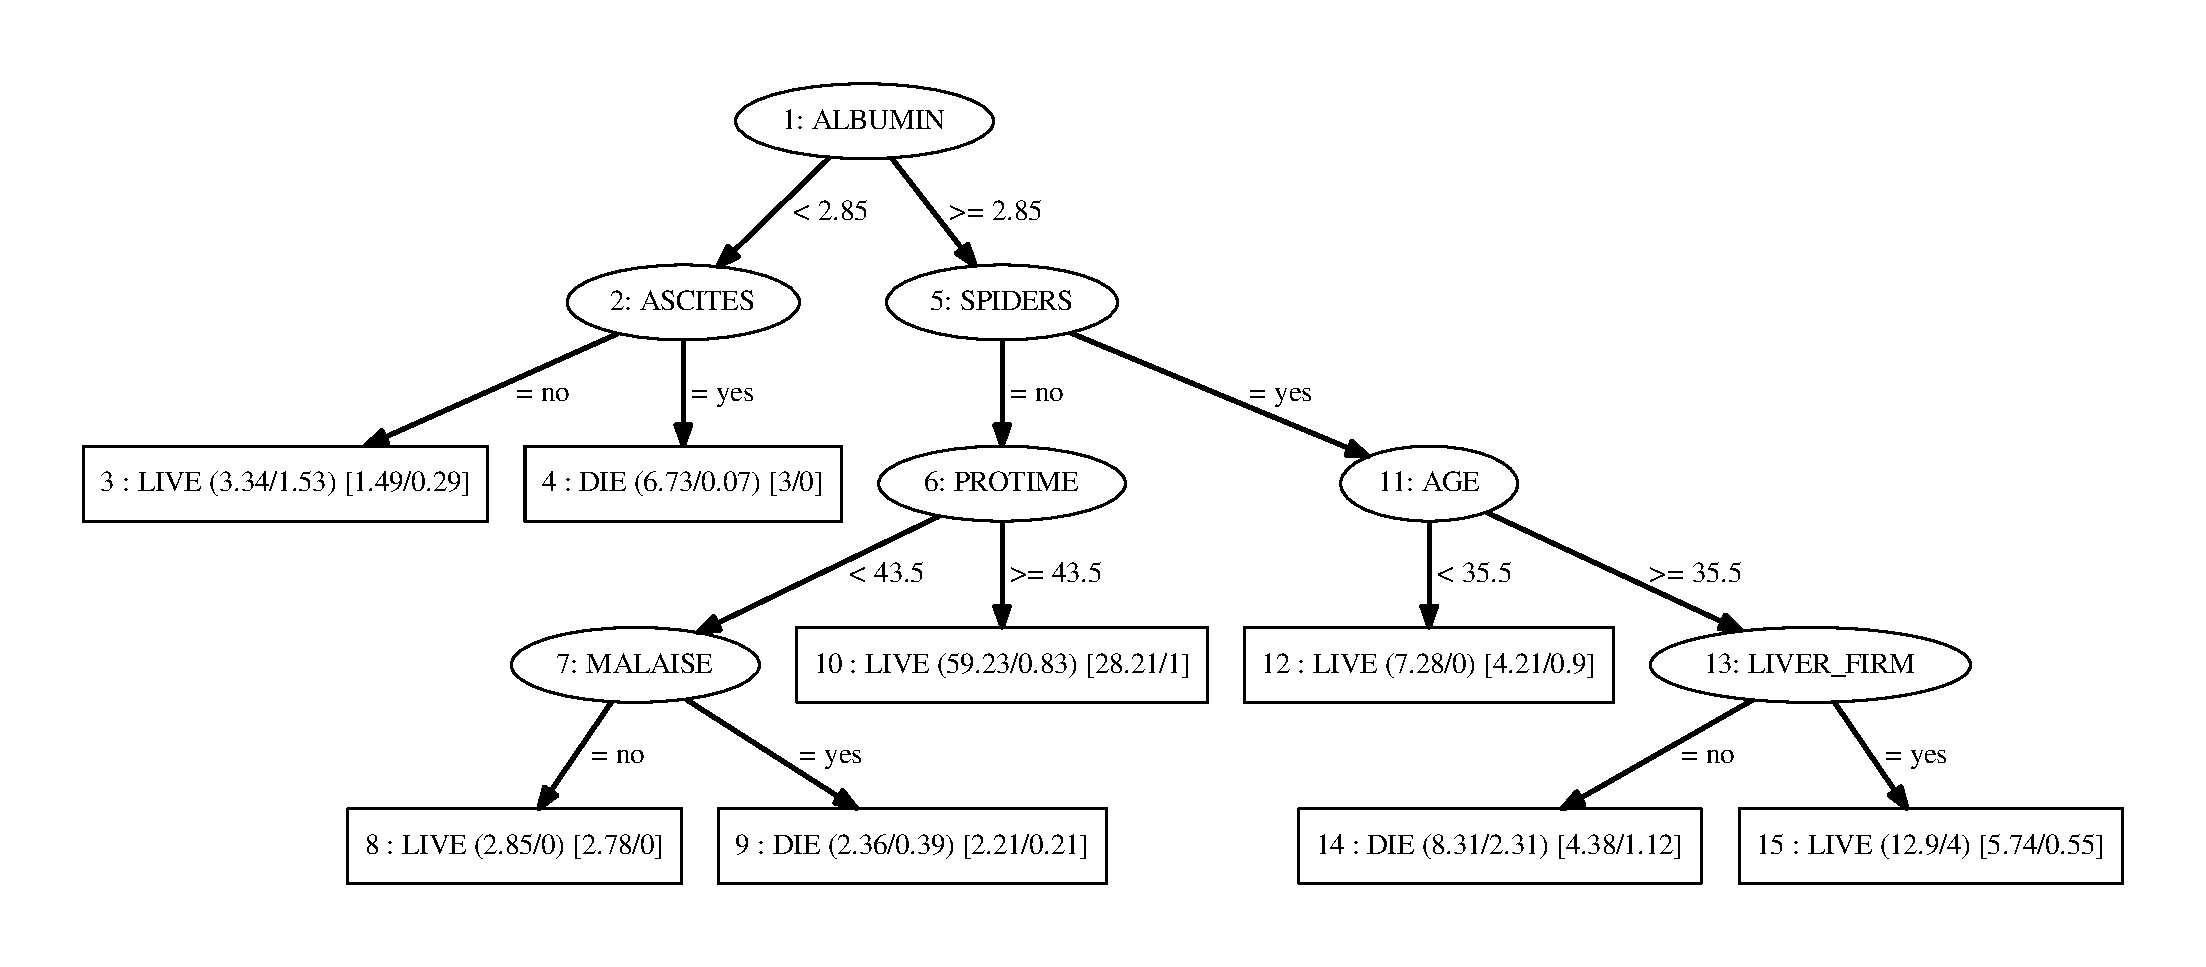
\includegraphics[width=1.55\textwidth]{results/reptree/hepatitis.pdf}}
	\caption{Modello di REPTree}
\end{figure}

\begin{mdframed}[frametitle=Esecuzione JRip]
	\footnotesize\verbatiminput{results/jrip/hepatitis.jrip}
\end{mdframed}


\noindent
\normalsize Regole:
\footnotesize\input{results/jrip/hepatitis.list.rules}

\pagebreak

\section{Risultati su \texttt{Vehicle Silhouettes}}

\normalsize L'esecuzione ha coinvolto 761 istanze di training e 85 istanze di testing ad ogni iterazione del CV.

\begin{mdframed}[frametitle=Esecuzione NaiveBayesSimple]
	\footnotesize\verbatiminput{results/nb/vehicle.nb}
\end{mdframed}


\scriptsize
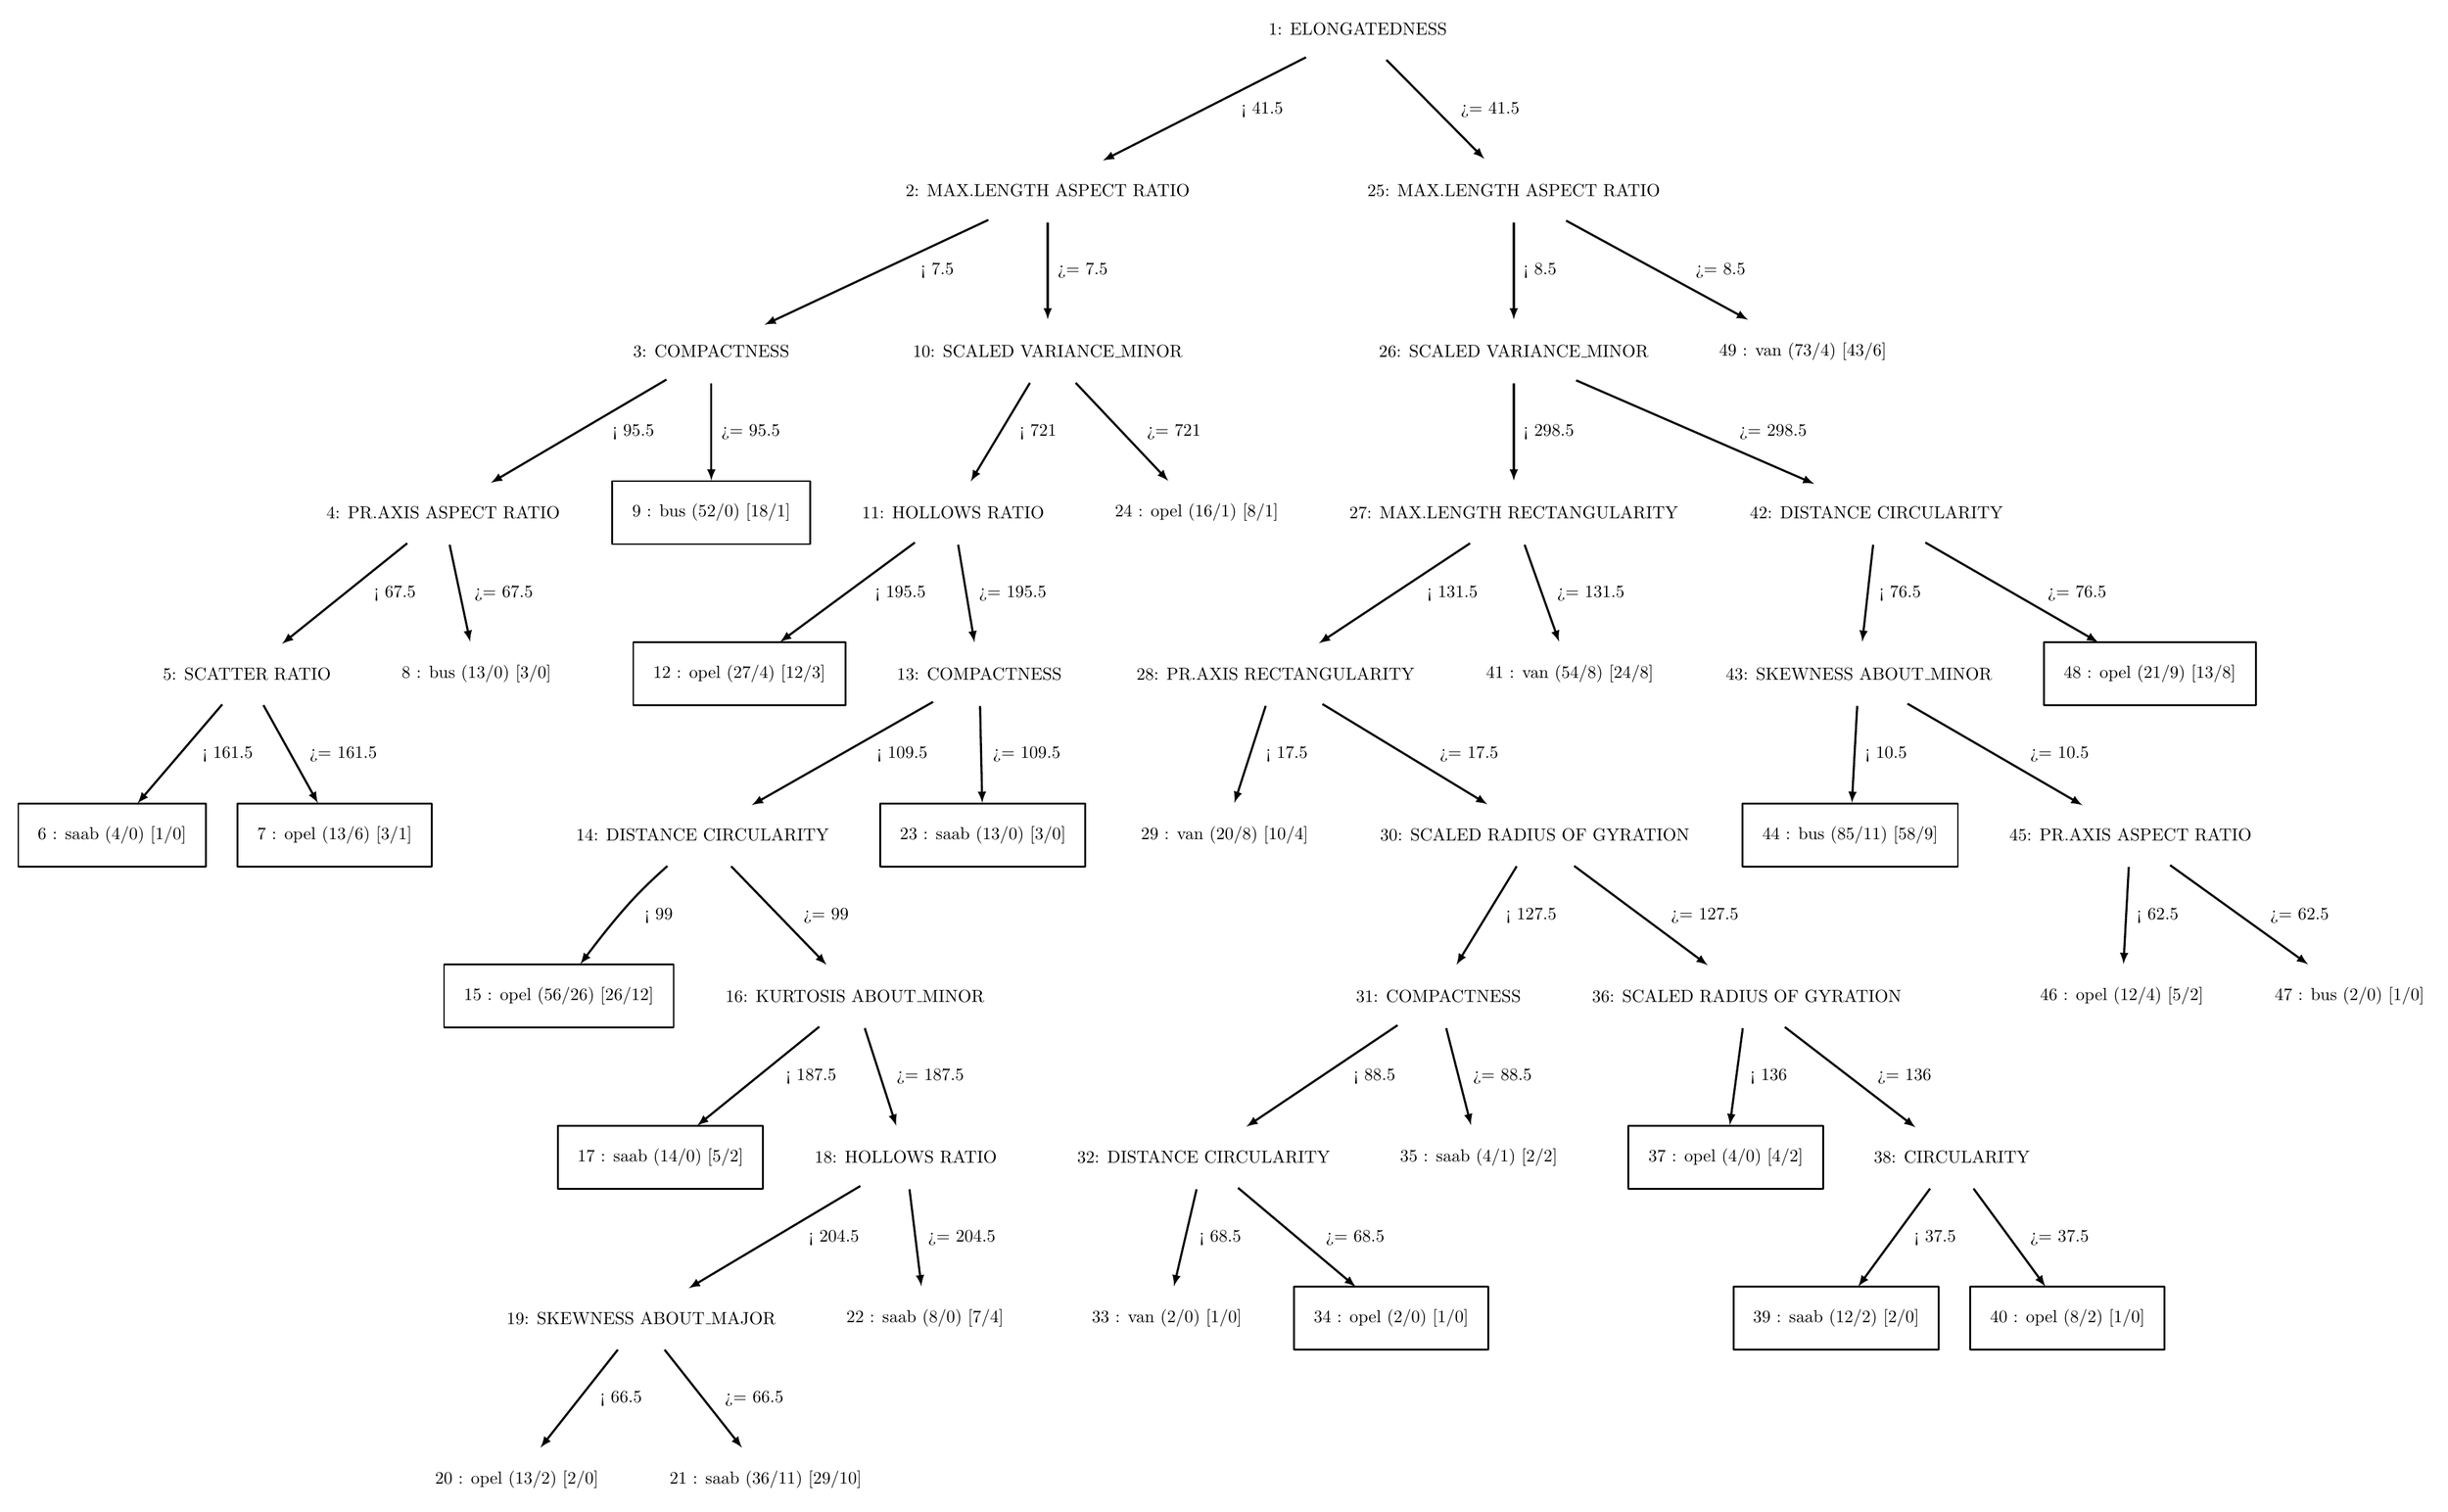
\begin{tikzpicture}[>=latex,line join=bevel,]
  \pgfsetlinewidth{1bp}
%%
\pgfsetcolor{black}
  % Edge: N4cdf35a9 -> N4c98385c
  \draw [->,very thick] (855.15bp,368.07bp) .. controls (847.01bp,354.75bp) and (835.53bp,335.95bp)  .. (820.8bp,311.85bp);
  \definecolor{strokecol}{rgb}{0.0,0.0,0.0};
  \pgfsetstrokecolor{strokecol}
  \draw (863.5bp,340.0bp) node { < 127.5};
  % Edge: N442d9b6e -> N15615099
  \draw [->,very thick] (1228.1bp,368.7bp) .. controls (1247.8bp,354.57bp) and (1276.4bp,333.96bp)  .. (1306.8bp,312.1bp);
  \draw (1302.0bp,340.0bp) node { >= 62.5};
  % Edge: N20fa23c1 -> N3581c5f3
  \draw [->,very thick] (221.96bp,552.49bp) .. controls (204.16bp,538.19bp) and (178.26bp,517.38bp)  .. (150.54bp,495.1bp);
  \draw (215.0bp,524.0bp) node { < 67.5};
  % Edge: N2b05039f -> N61e717c2
  \draw [->,very thick] (457.14bp,276.49bp) .. controls (439.84bp,262.46bp) and (414.79bp,242.15bp)  .. (387.48bp,220.01bp);
  \draw (452.5bp,248.0bp) node { < 187.5};
  % Edge: N484b61fc -> N45fe3ee3
  \draw [->,very thick] (711.91bp,459.65bp) .. controls (707.74bp,446.7bp) and (701.96bp,428.76bp)  .. (694.07bp,404.3bp);
  \draw (724.0bp,432.0bp) node { < 17.5};
  % Edge: N1a93a7ca -> N3d82c5f3
  \draw [->,very thick] (370.43bp,368.2bp) .. controls (364.15bp,362.63bp) and (357.34bp,356.25bp)  .. (351.5bp,350.0bp) .. controls (342.86bp,340.75bp) and (334.11bp,329.9bp)  .. (320.75bp,312.23bp);
  \draw (365.5bp,340.0bp) node { < 99};
  % Edge: N58d25a40 -> N1b701da1
  \draw [->,very thick] (1058.6bp,551.65bp) .. controls (1057.1bp,538.82bp) and (1055.2bp,521.11bp)  .. (1052.4bp,496.3bp);
  \draw (1074.0bp,524.0bp) node { < 76.5};
  % Edge: N4cdf35a9 -> N73a8dfcc
  \draw [->,very thick] (887.98bp,368.28bp) .. controls (907.16bp,354.01bp) and (934.93bp,333.36bp)  .. (964.14bp,311.63bp);
  \draw (962.5bp,340.0bp) node { >= 127.5};
  % Edge: N4dcbadb4 -> N17d10166
  \draw [->,very thick] (368.85bp,92.072bp) .. controls (379.5bp,78.581bp) and (394.56bp,59.486bp)  .. (412.96bp,36.158bp);
  \draw (420.0bp,64.0bp) node { >= 66.5};
  % Edge: N504bae78 -> N368102c8
  \draw [->,very thick] (883.38bp,736.7bp) .. controls (909.86bp,722.26bp) and (948.75bp,701.04bp)  .. (987.16bp,680.1bp);
  \draw (971.5bp,708.0bp) node { >= 8.5};
  % Edge: N3b764bce -> N759ebb3d
  \draw [->,very thick] (853.5bp,643.65bp) .. controls (853.5bp,630.82bp) and (853.5bp,613.11bp)  .. (853.5bp,588.3bp);
  \draw (873.5bp,616.0bp) node { < 298.5};
  % Edge: N73a8dfcc -> N7e774085
  \draw [->,very thick] (1008.2bp,276.28bp) .. controls (1026.9bp,261.9bp) and (1054.1bp,241.02bp)  .. (1082.7bp,219.02bp);
  \draw (1076.5bp,248.0bp) node { >= 136};
  % Edge: N3b764bce -> N58d25a40
  \draw [->,very thick] (889.08bp,645.53bp) .. controls (924.14bp,630.29bp) and (977.82bp,606.95bp)  .. (1025.0bp,586.42bp);
  \draw (1001.5bp,616.0bp) node { >= 298.5};
  % Edge: N593634ad -> N20fa23c1
  \draw [->,very thick] (369.89bp,645.94bp) .. controls (344.87bp,631.22bp) and (306.55bp,608.67bp)  .. (269.74bp,587.02bp);
  \draw (351.0bp,616.0bp) node { < 95.5};
  % Edge: N7506e922 -> N504bae78
  \draw [->,very thick] (780.82bp,828.49bp) .. controls (794.45bp,814.71bp) and (814.07bp,794.87bp)  .. (836.67bp,772.01bp);
  \draw (840.0bp,800.0bp) node { >= 41.5};
  % Edge: N20fa23c1 -> N73c6c3b2
  \draw [->,very thick] (246.16bp,551.65bp) .. controls (248.87bp,538.82bp) and (252.61bp,521.11bp)  .. (257.85bp,496.3bp);
  \draw (277.0bp,524.0bp) node { >= 67.5};
  % Edge: N7e0b37bc -> N6ae40994
  \draw [->,very thick] (536.39bp,551.65bp) .. controls (538.54bp,538.74bp) and (541.52bp,520.88bp)  .. (545.67bp,495.99bp);
  \draw (567.5bp,524.0bp) node { >= 195.5};
  % Edge: N593634ad -> N48533e64
  \draw [->,very thick] (395.5bp,643.65bp) .. controls (395.5bp,630.82bp) and (395.5bp,613.11bp)  .. (395.5bp,588.3bp);
  \draw (418.0bp,616.0bp) node { >= 95.5};
  % Edge: N73a8dfcc -> Nea30797
  \draw [->,very thick] (984.19bp,275.65bp) .. controls (982.48bp,262.82bp) and (980.11bp,245.11bp)  .. (976.81bp,220.3bp);
  \draw (999.0bp,248.0bp) node { < 136};
  % Edge: N442d9b6e -> Nee7d9f1
  \draw [->,very thick] (1204.5bp,367.65bp) .. controls (1203.8bp,354.82bp) and (1202.8bp,337.11bp)  .. (1201.5bp,312.3bp);
  \draw (1221.0bp,340.0bp) node { < 62.5};
  % Edge: N5fcfe4b2 -> N5eb5c224
  \draw [->,very thick] (696.13bp,184.49bp) .. controls (712.73bp,170.52bp) and (736.74bp,150.33bp)  .. (763.27bp,128.01bp);
  \draw (763.0bp,156.0bp) node { >= 68.5};
  % Edge: N2b05039f -> N66cd51c3
  \draw [->,very thick] (483.09bp,275.65bp) .. controls (487.29bp,262.62bp) and (493.12bp,244.53bp)  .. (501.02bp,219.99bp);
  \draw (520.5bp,248.0bp) node { >= 187.5};
  % Edge: N7e774085 -> N3f8f9dd6
  \draw [->,very thick] (1091.1bp,184.07bp) .. controls (1081.3bp,170.71bp) and (1067.4bp,151.84bp)  .. (1050.1bp,128.16bp);
  \draw (1094.0bp,156.0bp) node { < 37.5};
  % Edge: N66cd51c3 -> N1b9e1916
  \draw [->,very thick] (508.62bp,183.65bp) .. controls (510.19bp,170.82bp) and (512.35bp,153.11bp)  .. (515.39bp,128.3bp);
  \draw (538.5bp,156.0bp) node { >= 204.5};
  % Edge: N64a294a6 -> N4f8e5cde
  \draw [->,very thick] (603.49bp,644.07bp) .. controls (616.35bp,630.46bp) and (634.6bp,611.13bp)  .. (656.29bp,588.16bp);
  \draw (659.5bp,616.0bp) node { >= 721};
  % Edge: N4ee285c6 -> N593634ad
  \draw [->,very thick] (553.62bp,737.12bp) .. controls (520.55bp,721.62bp) and (470.26bp,698.04bp)  .. (425.88bp,677.24bp);
  \draw (524.5bp,708.0bp) node { < 7.5};
  % Edge: N484b61fc -> N4cdf35a9
  \draw [->,very thick] (744.3bp,460.7bp) .. controls (768.25bp,446.14bp) and (803.52bp,424.69bp)  .. (838.4bp,403.48bp);
  \draw (828.0bp,432.0bp) node { >= 17.5};
  % Edge: N3581c5f3 -> N6aa8ceb6
  \draw [->,very thick] (116.38bp,460.49bp) .. controls (104.69bp,446.84bp) and (87.923bp,427.23bp)  .. (68.057bp,404.01bp);
  \draw (119.5bp,432.0bp) node { < 161.5};
  % Edge: N7e774085 -> Naec6354
  \draw [->,very thick] (1115.9bp,184.07bp) .. controls (1125.7bp,170.71bp) and (1139.6bp,151.84bp)  .. (1156.9bp,128.16bp);
  \draw (1165.0bp,156.0bp) node { >= 37.5};
  % Edge: N58d25a40 -> N1edf1c96
  \draw [->,very thick] (1088.4bp,552.91bp) .. controls (1113.5bp,538.45bp) and (1150.5bp,517.08bp)  .. (1187.0bp,496.02bp);
  \draw (1175.0bp,524.0bp) node { >= 76.5};
  % Edge: N3581c5f3 -> N2530c12
  \draw [->,very thick] (139.9bp,460.07bp) .. controls (147.26bp,446.83bp) and (157.62bp,428.19bp)  .. (170.97bp,404.16bp);
  \draw (185.5bp,432.0bp) node { >= 161.5};
  % Edge: N64a294a6 -> N7e0b37bc
  \draw [->,very thick] (577.34bp,644.07bp) .. controls (569.35bp,630.75bp) and (558.07bp,611.95bp)  .. (543.61bp,587.85bp);
  \draw (582.0bp,616.0bp) node { < 721};
  % Edge: N4c98385c -> N53e25b76
  \draw [->,very thick] (814.93bp,275.65bp) .. controls (818.21bp,262.82bp) and (822.74bp,245.11bp)  .. (829.08bp,220.3bp);
  \draw (847.0bp,248.0bp) node { >= 88.5};
  % Edge: N759ebb3d -> N484b61fc
  \draw [->,very thick] (828.56bp,552.49bp) .. controls (806.7bp,538.03bp) and (774.77bp,516.9bp)  .. (742.29bp,495.4bp);
  \draw (818.5bp,524.0bp) node { < 131.5};
  % Edge: N5fcfe4b2 -> N6bf2d08e
  \draw [->,very thick] (672.45bp,183.65bp) .. controls (669.46bp,170.82bp) and (665.33bp,153.11bp)  .. (659.54bp,128.3bp);
  \draw (686.0bp,156.0bp) node { < 68.5};
  % Edge: N504bae78 -> N3b764bce
  \draw [->,very thick] (853.5bp,735.65bp) .. controls (853.5bp,722.82bp) and (853.5bp,705.11bp)  .. (853.5bp,680.3bp);
  \draw (868.5bp,708.0bp) node { < 8.5};
  % Edge: N4ee285c6 -> N64a294a6
  \draw [->,very thick] (587.5bp,735.65bp) .. controls (587.5bp,722.82bp) and (587.5bp,705.11bp)  .. (587.5bp,680.3bp);
  \draw (607.5bp,708.0bp) node { >= 7.5};
  % Edge: N6ae40994 -> N1a93a7ca
  \draw [->,very thick] (522.05bp,461.94bp) .. controls (496.21bp,447.22bp) and (456.64bp,424.67bp)  .. (418.63bp,403.02bp);
  \draw (504.5bp,432.0bp) node { < 109.5};
  % Edge: N1b701da1 -> N726f3b58
  \draw [->,very thick] (1049.5bp,459.65bp) .. controls (1048.8bp,446.82bp) and (1047.8bp,429.11bp)  .. (1046.5bp,404.3bp);
  \draw (1066.0bp,432.0bp) node { < 10.5};
  % Edge: N4c98385c -> N5fcfe4b2
  \draw [->,very thick] (787.16bp,277.32bp) .. controls (765.65bp,262.88bp) and (733.52bp,241.3bp)  .. (700.93bp,219.41bp);
  \draw (774.0bp,248.0bp) node { < 88.5};
  % Edge: N4dcbadb4 -> N4e515669
  \draw [->,very thick] (342.15bp,92.072bp) .. controls (331.5bp,78.581bp) and (316.44bp,59.486bp)  .. (298.04bp,36.158bp);
  \draw (344.0bp,64.0bp) node { < 66.5};
  % Edge: N759ebb3d -> N1c655221
  \draw [->,very thick] (859.67bp,551.65bp) .. controls (864.27bp,538.7bp) and (870.65bp,520.76bp)  .. (879.35bp,496.3bp);
  \draw (897.5bp,524.0bp) node { >= 131.5};
  % Edge: N6ae40994 -> Nba8a1dc
  \draw [->,very thick] (548.89bp,459.65bp) .. controls (549.17bp,446.82bp) and (549.56bp,429.11bp)  .. (550.12bp,404.3bp);
  \draw (575.5bp,432.0bp) node { >= 109.5};
  % Edge: N66cd51c3 -> N4dcbadb4
  \draw [->,very thick] (480.54bp,185.53bp) .. controls (456.0bp,170.9bp) and (418.94bp,148.81bp)  .. (382.65bp,127.18bp);
  \draw (465.5bp,156.0bp) node { < 204.5};
  % Edge: N1b701da1 -> N442d9b6e
  \draw [->,very thick] (1078.2bp,460.91bp) .. controls (1103.7bp,446.13bp) and (1141.6bp,424.13bp)  .. (1178.0bp,402.95bp);
  \draw (1165.0bp,432.0bp) node { >= 10.5};
  % Edge: N7e0b37bc -> N3b95a09c
  \draw [->,very thick] (511.69bp,552.91bp) .. controls (492.57bp,538.8bp) and (464.54bp,518.13bp)  .. (434.78bp,496.18bp);
  \draw (503.5bp,524.0bp) node { < 195.5};
  % Edge: N7506e922 -> N4ee285c6
  \draw [->,very thick] (734.87bp,829.94bp) .. controls (705.67bp,815.09bp) and (660.82bp,792.28bp)  .. (619.01bp,771.02bp);
  \draw (710.0bp,800.0bp) node { < 41.5};
  % Edge: N1a93a7ca -> N2b05039f
  \draw [->,very thick] (406.86bp,368.07bp) .. controls (420.23bp,354.24bp) and (439.29bp,334.53bp)  .. (461.21bp,311.85bp);
  \draw (461.0bp,340.0bp) node { >= 99};
  % Node: N2b05039f
\begin{scope}
  \definecolor{strokecol}{rgb}{0.0,0.0,0.0};
  \pgfsetstrokecolor{strokecol}
  \draw (477.5bp,294.0bp) node {16: KURTOSIS ABOUT\_MINOR};
\end{scope}
  % Node: N1b701da1
\begin{scope}
  \definecolor{strokecol}{rgb}{0.0,0.0,0.0};
  \pgfsetstrokecolor{strokecol}
  \draw (1050.5bp,478.0bp) node {43: SKEWNESS ABOUT\_MINOR};
\end{scope}
  % Node: N4e515669
\begin{scope}
  \definecolor{strokecol}{rgb}{0.0,0.0,0.0};
  \pgfsetstrokecolor{strokecol}
  \draw (284.5bp,18.0bp) node {20 : opel (13/2) [2/0]};
\end{scope}
  % Node: N17d10166
\begin{scope}
  \definecolor{strokecol}{rgb}{0.0,0.0,0.0};
  \pgfsetstrokecolor{strokecol}
  \draw (426.5bp,18.0bp) node {21 : saab (36/11) [29/10]};
\end{scope}
  % Node: N6aa8ceb6
\begin{scope}
  \definecolor{strokecol}{rgb}{0.0,0.0,0.0};
  \pgfsetstrokecolor{strokecol}
  \draw (107.0bp,404.0bp) -- (0.0bp,404.0bp) -- (0.0bp,368.0bp) -- (107.0bp,368.0bp) -- cycle;
  \draw (53.5bp,386.0bp) node {6 : saab (4/0) [1/0]};
\end{scope}
  % Node: N1a93a7ca
\begin{scope}
  \definecolor{strokecol}{rgb}{0.0,0.0,0.0};
  \pgfsetstrokecolor{strokecol}
  \draw (390.5bp,386.0bp) node {14: DISTANCE CIRCULARITY};
\end{scope}
  % Node: N4ee285c6
\begin{scope}
  \definecolor{strokecol}{rgb}{0.0,0.0,0.0};
  \pgfsetstrokecolor{strokecol}
  \draw (587.5bp,754.0bp) node {2: MAX.LENGTH ASPECT RATIO};
\end{scope}
  % Node: N66cd51c3
\begin{scope}
  \definecolor{strokecol}{rgb}{0.0,0.0,0.0};
  \pgfsetstrokecolor{strokecol}
  \draw (506.5bp,202.0bp) node {18: HOLLOWS RATIO};
\end{scope}
  % Node: N5eb5c224
\begin{scope}
  \definecolor{strokecol}{rgb}{0.0,0.0,0.0};
  \pgfsetstrokecolor{strokecol}
  \draw (839.0bp,128.0bp) -- (728.0bp,128.0bp) -- (728.0bp,92.0bp) -- (839.0bp,92.0bp) -- cycle;
  \draw (783.5bp,110.0bp) node {34 : opel (2/0) [1/0]};
\end{scope}
  % Node: Nee7d9f1
\begin{scope}
  \definecolor{strokecol}{rgb}{0.0,0.0,0.0};
  \pgfsetstrokecolor{strokecol}
  \draw (1200.5bp,294.0bp) node {46 : opel (12/4) [5/2]};
\end{scope}
  % Node: N368102c8
\begin{scope}
  \definecolor{strokecol}{rgb}{0.0,0.0,0.0};
  \pgfsetstrokecolor{strokecol}
  \draw (1018.5bp,662.0bp) node {49 : van (73/4) [43/6]};
\end{scope}
  % Node: N1c655221
\begin{scope}
  \definecolor{strokecol}{rgb}{0.0,0.0,0.0};
  \pgfsetstrokecolor{strokecol}
  \draw (885.5bp,478.0bp) node {41 : van (54/8) [24/8]};
\end{scope}
  % Node: N7e0b37bc
\begin{scope}
  \definecolor{strokecol}{rgb}{0.0,0.0,0.0};
  \pgfsetstrokecolor{strokecol}
  \draw (533.5bp,570.0bp) node {11: HOLLOWS RATIO};
\end{scope}
  % Node: Naec6354
\begin{scope}
  \definecolor{strokecol}{rgb}{0.0,0.0,0.0};
  \pgfsetstrokecolor{strokecol}
  \draw (1225.0bp,128.0bp) -- (1114.0bp,128.0bp) -- (1114.0bp,92.0bp) -- (1225.0bp,92.0bp) -- cycle;
  \draw (1169.5bp,110.0bp) node {40 : opel (8/2) [1/0]};
\end{scope}
  % Node: N2530c12
\begin{scope}
  \definecolor{strokecol}{rgb}{0.0,0.0,0.0};
  \pgfsetstrokecolor{strokecol}
  \draw (236.0bp,404.0bp) -- (125.0bp,404.0bp) -- (125.0bp,368.0bp) -- (236.0bp,368.0bp) -- cycle;
  \draw (180.5bp,386.0bp) node {7 : opel (13/6) [3/1]};
\end{scope}
  % Node: N504bae78
\begin{scope}
  \definecolor{strokecol}{rgb}{0.0,0.0,0.0};
  \pgfsetstrokecolor{strokecol}
  \draw (853.5bp,754.0bp) node {25: MAX.LENGTH ASPECT RATIO};
\end{scope}
  % Node: N484b61fc
\begin{scope}
  \definecolor{strokecol}{rgb}{0.0,0.0,0.0};
  \pgfsetstrokecolor{strokecol}
  \draw (717.5bp,478.0bp) node {28: PR.AXIS RECTANGULARITY};
\end{scope}
  % Node: N1edf1c96
\begin{scope}
  \definecolor{strokecol}{rgb}{0.0,0.0,0.0};
  \pgfsetstrokecolor{strokecol}
  \draw (1277.0bp,496.0bp) -- (1156.0bp,496.0bp) -- (1156.0bp,460.0bp) -- (1277.0bp,460.0bp) -- cycle;
  \draw (1216.5bp,478.0bp) node {48 : opel (21/9) [13/8]};
\end{scope}
  % Node: N4c98385c
\begin{scope}
  \definecolor{strokecol}{rgb}{0.0,0.0,0.0};
  \pgfsetstrokecolor{strokecol}
  \draw (810.5bp,294.0bp) node {31: COMPACTNESS};
\end{scope}
  % Node: N45fe3ee3
\begin{scope}
  \definecolor{strokecol}{rgb}{0.0,0.0,0.0};
  \pgfsetstrokecolor{strokecol}
  \draw (688.5bp,386.0bp) node {29 : van (20/8) [10/4]};
\end{scope}
  % Node: N726f3b58
\begin{scope}
  \definecolor{strokecol}{rgb}{0.0,0.0,0.0};
  \pgfsetstrokecolor{strokecol}
  \draw (1107.0bp,404.0bp) -- (984.0bp,404.0bp) -- (984.0bp,368.0bp) -- (1107.0bp,368.0bp) -- cycle;
  \draw (1045.5bp,386.0bp) node {44 : bus (85/11) [58/9]};
\end{scope}
  % Node: N4cdf35a9
\begin{scope}
  \definecolor{strokecol}{rgb}{0.0,0.0,0.0};
  \pgfsetstrokecolor{strokecol}
  \draw (865.5bp,386.0bp) node {30: SCALED RADIUS OF GYRATION};
\end{scope}
  % Node: N5fcfe4b2
\begin{scope}
  \definecolor{strokecol}{rgb}{0.0,0.0,0.0};
  \pgfsetstrokecolor{strokecol}
  \draw (676.5bp,202.0bp) node {32: DISTANCE CIRCULARITY};
\end{scope}
  % Node: N15615099
\begin{scope}
  \definecolor{strokecol}{rgb}{0.0,0.0,0.0};
  \pgfsetstrokecolor{strokecol}
  \draw (1330.5bp,294.0bp) node {47 : bus (2/0) [1/0]};
\end{scope}
  % Node: N442d9b6e
\begin{scope}
  \definecolor{strokecol}{rgb}{0.0,0.0,0.0};
  \pgfsetstrokecolor{strokecol}
  \draw (1205.5bp,386.0bp) node {45: PR.AXIS ASPECT RATIO};
\end{scope}
  % Node: N6bf2d08e
\begin{scope}
  \definecolor{strokecol}{rgb}{0.0,0.0,0.0};
  \pgfsetstrokecolor{strokecol}
  \draw (655.5bp,110.0bp) node {33 : van (2/0) [1/0]};
\end{scope}
  % Node: N3b764bce
\begin{scope}
  \definecolor{strokecol}{rgb}{0.0,0.0,0.0};
  \pgfsetstrokecolor{strokecol}
  \draw (853.5bp,662.0bp) node {26: SCALED VARIANCE\_MINOR};
\end{scope}
  % Node: N64a294a6
\begin{scope}
  \definecolor{strokecol}{rgb}{0.0,0.0,0.0};
  \pgfsetstrokecolor{strokecol}
  \draw (587.5bp,662.0bp) node {10: SCALED VARIANCE\_MINOR};
\end{scope}
  % Node: N3581c5f3
\begin{scope}
  \definecolor{strokecol}{rgb}{0.0,0.0,0.0};
  \pgfsetstrokecolor{strokecol}
  \draw (130.5bp,478.0bp) node {5: SCATTER RATIO};
\end{scope}
  % Node: Nba8a1dc
\begin{scope}
  \definecolor{strokecol}{rgb}{0.0,0.0,0.0};
  \pgfsetstrokecolor{strokecol}
  \draw (609.0bp,404.0bp) -- (492.0bp,404.0bp) -- (492.0bp,368.0bp) -- (609.0bp,368.0bp) -- cycle;
  \draw (550.5bp,386.0bp) node {23 : saab (13/0) [3/0]};
\end{scope}
  % Node: N58d25a40
\begin{scope}
  \definecolor{strokecol}{rgb}{0.0,0.0,0.0};
  \pgfsetstrokecolor{strokecol}
  \draw (1060.5bp,570.0bp) node {42: DISTANCE CIRCULARITY};
\end{scope}
  % Node: N48533e64
\begin{scope}
  \definecolor{strokecol}{rgb}{0.0,0.0,0.0};
  \pgfsetstrokecolor{strokecol}
  \draw (452.0bp,588.0bp) -- (339.0bp,588.0bp) -- (339.0bp,552.0bp) -- (452.0bp,552.0bp) -- cycle;
  \draw (395.5bp,570.0bp) node {9 : bus (52/0) [18/1]};
\end{scope}
  % Node: N759ebb3d
\begin{scope}
  \definecolor{strokecol}{rgb}{0.0,0.0,0.0};
  \pgfsetstrokecolor{strokecol}
  \draw (853.5bp,570.0bp) node {27: MAX.LENGTH RECTANGULARITY};
\end{scope}
  % Node: N1b9e1916
\begin{scope}
  \definecolor{strokecol}{rgb}{0.0,0.0,0.0};
  \pgfsetstrokecolor{strokecol}
  \draw (517.5bp,110.0bp) node {22 : saab (8/0) [7/4]};
\end{scope}
  % Node: N4f8e5cde
\begin{scope}
  \definecolor{strokecol}{rgb}{0.0,0.0,0.0};
  \pgfsetstrokecolor{strokecol}
  \draw (672.5bp,570.0bp) node {24 : opel (16/1) [8/1]};
\end{scope}
  % Node: N20fa23c1
\begin{scope}
  \definecolor{strokecol}{rgb}{0.0,0.0,0.0};
  \pgfsetstrokecolor{strokecol}
  \draw (242.5bp,570.0bp) node {4: PR.AXIS ASPECT RATIO};
\end{scope}
  % Node: N73c6c3b2
\begin{scope}
  \definecolor{strokecol}{rgb}{0.0,0.0,0.0};
  \pgfsetstrokecolor{strokecol}
  \draw (261.5bp,478.0bp) node {8 : bus (13/0) [3/0]};
\end{scope}
  % Node: N73a8dfcc
\begin{scope}
  \definecolor{strokecol}{rgb}{0.0,0.0,0.0};
  \pgfsetstrokecolor{strokecol}
  \draw (986.5bp,294.0bp) node {36: SCALED RADIUS OF GYRATION};
\end{scope}
  % Node: N4dcbadb4
\begin{scope}
  \definecolor{strokecol}{rgb}{0.0,0.0,0.0};
  \pgfsetstrokecolor{strokecol}
  \draw (355.5bp,110.0bp) node {19: SKEWNESS ABOUT\_MAJOR};
\end{scope}
  % Node: N6ae40994
\begin{scope}
  \definecolor{strokecol}{rgb}{0.0,0.0,0.0};
  \pgfsetstrokecolor{strokecol}
  \draw (548.5bp,478.0bp) node {13: COMPACTNESS};
\end{scope}
  % Node: N3f8f9dd6
\begin{scope}
  \definecolor{strokecol}{rgb}{0.0,0.0,0.0};
  \pgfsetstrokecolor{strokecol}
  \draw (1096.0bp,128.0bp) -- (979.0bp,128.0bp) -- (979.0bp,92.0bp) -- (1096.0bp,92.0bp) -- cycle;
  \draw (1037.5bp,110.0bp) node {39 : saab (12/2) [2/0]};
\end{scope}
  % Node: N7e774085
\begin{scope}
  \definecolor{strokecol}{rgb}{0.0,0.0,0.0};
  \pgfsetstrokecolor{strokecol}
  \draw (1103.5bp,202.0bp) node {38: CIRCULARITY};
\end{scope}
  % Node: N61e717c2
\begin{scope}
  \definecolor{strokecol}{rgb}{0.0,0.0,0.0};
  \pgfsetstrokecolor{strokecol}
  \draw (425.0bp,220.0bp) -- (308.0bp,220.0bp) -- (308.0bp,184.0bp) -- (425.0bp,184.0bp) -- cycle;
  \draw (366.5bp,202.0bp) node {17 : saab (14/0) [5/2]};
\end{scope}
  % Node: N53e25b76
\begin{scope}
  \definecolor{strokecol}{rgb}{0.0,0.0,0.0};
  \pgfsetstrokecolor{strokecol}
  \draw (833.5bp,202.0bp) node {35 : saab (4/1) [2/2]};
\end{scope}
  % Node: N7506e922
\begin{scope}
  \definecolor{strokecol}{rgb}{0.0,0.0,0.0};
  \pgfsetstrokecolor{strokecol}
  \draw (764.5bp,846.0bp) node {1: ELONGATEDNESS};
\end{scope}
  % Node: N593634ad
\begin{scope}
  \definecolor{strokecol}{rgb}{0.0,0.0,0.0};
  \pgfsetstrokecolor{strokecol}
  \draw (395.5bp,662.0bp) node {3: COMPACTNESS};
\end{scope}
  % Node: N3b95a09c
\begin{scope}
  \definecolor{strokecol}{rgb}{0.0,0.0,0.0};
  \pgfsetstrokecolor{strokecol}
  \draw (472.0bp,496.0bp) -- (351.0bp,496.0bp) -- (351.0bp,460.0bp) -- (472.0bp,460.0bp) -- cycle;
  \draw (411.5bp,478.0bp) node {12 : opel (27/4) [12/3]};
\end{scope}
  % Node: Nea30797
\begin{scope}
  \definecolor{strokecol}{rgb}{0.0,0.0,0.0};
  \pgfsetstrokecolor{strokecol}
  \draw (1030.0bp,220.0bp) -- (919.0bp,220.0bp) -- (919.0bp,184.0bp) -- (1030.0bp,184.0bp) -- cycle;
  \draw (974.5bp,202.0bp) node {37 : opel (4/0) [4/2]};
\end{scope}
  % Node: N3d82c5f3
\begin{scope}
  \definecolor{strokecol}{rgb}{0.0,0.0,0.0};
  \pgfsetstrokecolor{strokecol}
  \draw (374.0bp,312.0bp) -- (243.0bp,312.0bp) -- (243.0bp,276.0bp) -- (374.0bp,276.0bp) -- cycle;
  \draw (308.5bp,294.0bp) node {15 : opel (56/26) [26/12]};
\end{scope}
%
\end{tikzpicture}



\begin{mdframed}[frametitle=Esecuzione REPTree]
	\scriptsize\verbatiminput{results/reptree/vehicle.reptree}
\end{mdframed}


\begin{figure}[htb]
	\makebox[\textwidth]{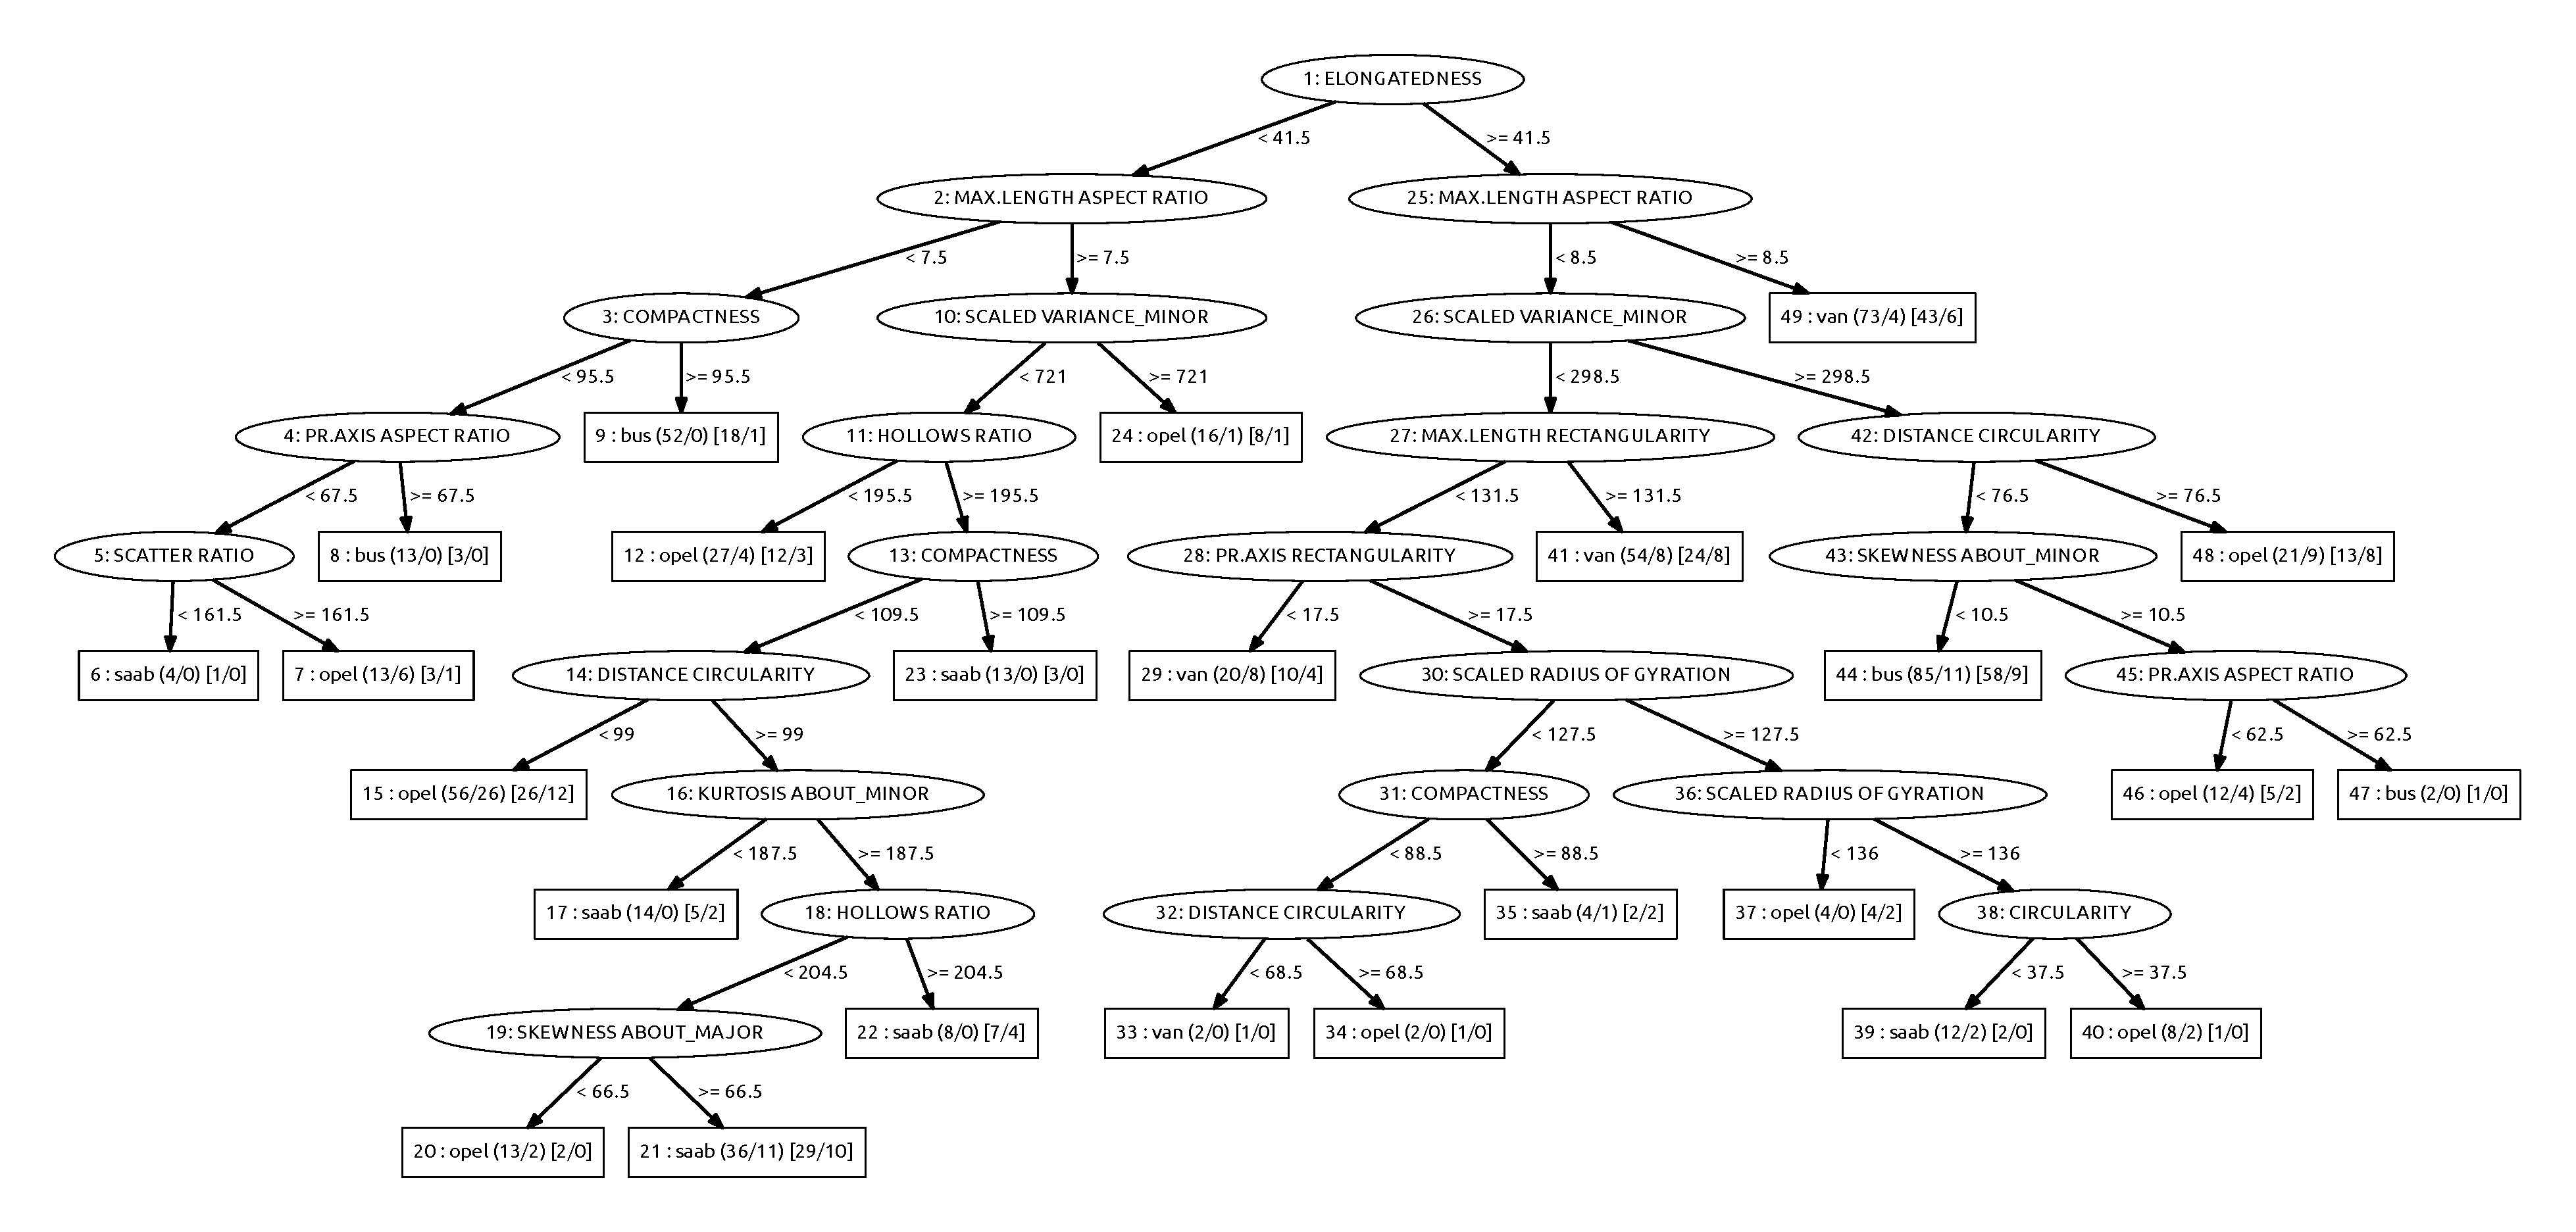
\includegraphics[width=1.55\textwidth]{results/reptree/vehicle.pdf}}
	\caption{Modello di REPTree}
\end{figure}

\begin{mdframed}[frametitle=Esecuzione JRip]
	\scriptsize\verbatiminput{results/jrip/vehicle.jrip}
\end{mdframed}


\noindent
\normalsize Regole:
\scriptsize\input{results/jrip/vehicle.list.rules}

\pagebreak

\section{Risultati su \texttt{Wisconsin Breast Cancer}}

\normalsize L'esecuzione ha coinvolto 629 istanze di training e 70 istanze di testing per ogni fold.


\begin{mdframed}[frametitle=Esecuzione NaiveBayesSimple]
	\footnotesize\verbatiminput{results/nb/wbc.nb}
\end{mdframed}


\footnotesize\input{results/nb/wbc.nbc}

\begin{mdframed}[frametitle=Esecuzione REPTree]
	\footnotesize\verbatiminput{results/reptree/wisconsin_breast_cancer.reptree}
\end{mdframed}


\begin{figure}[htb]
	\makebox[\textwidth]{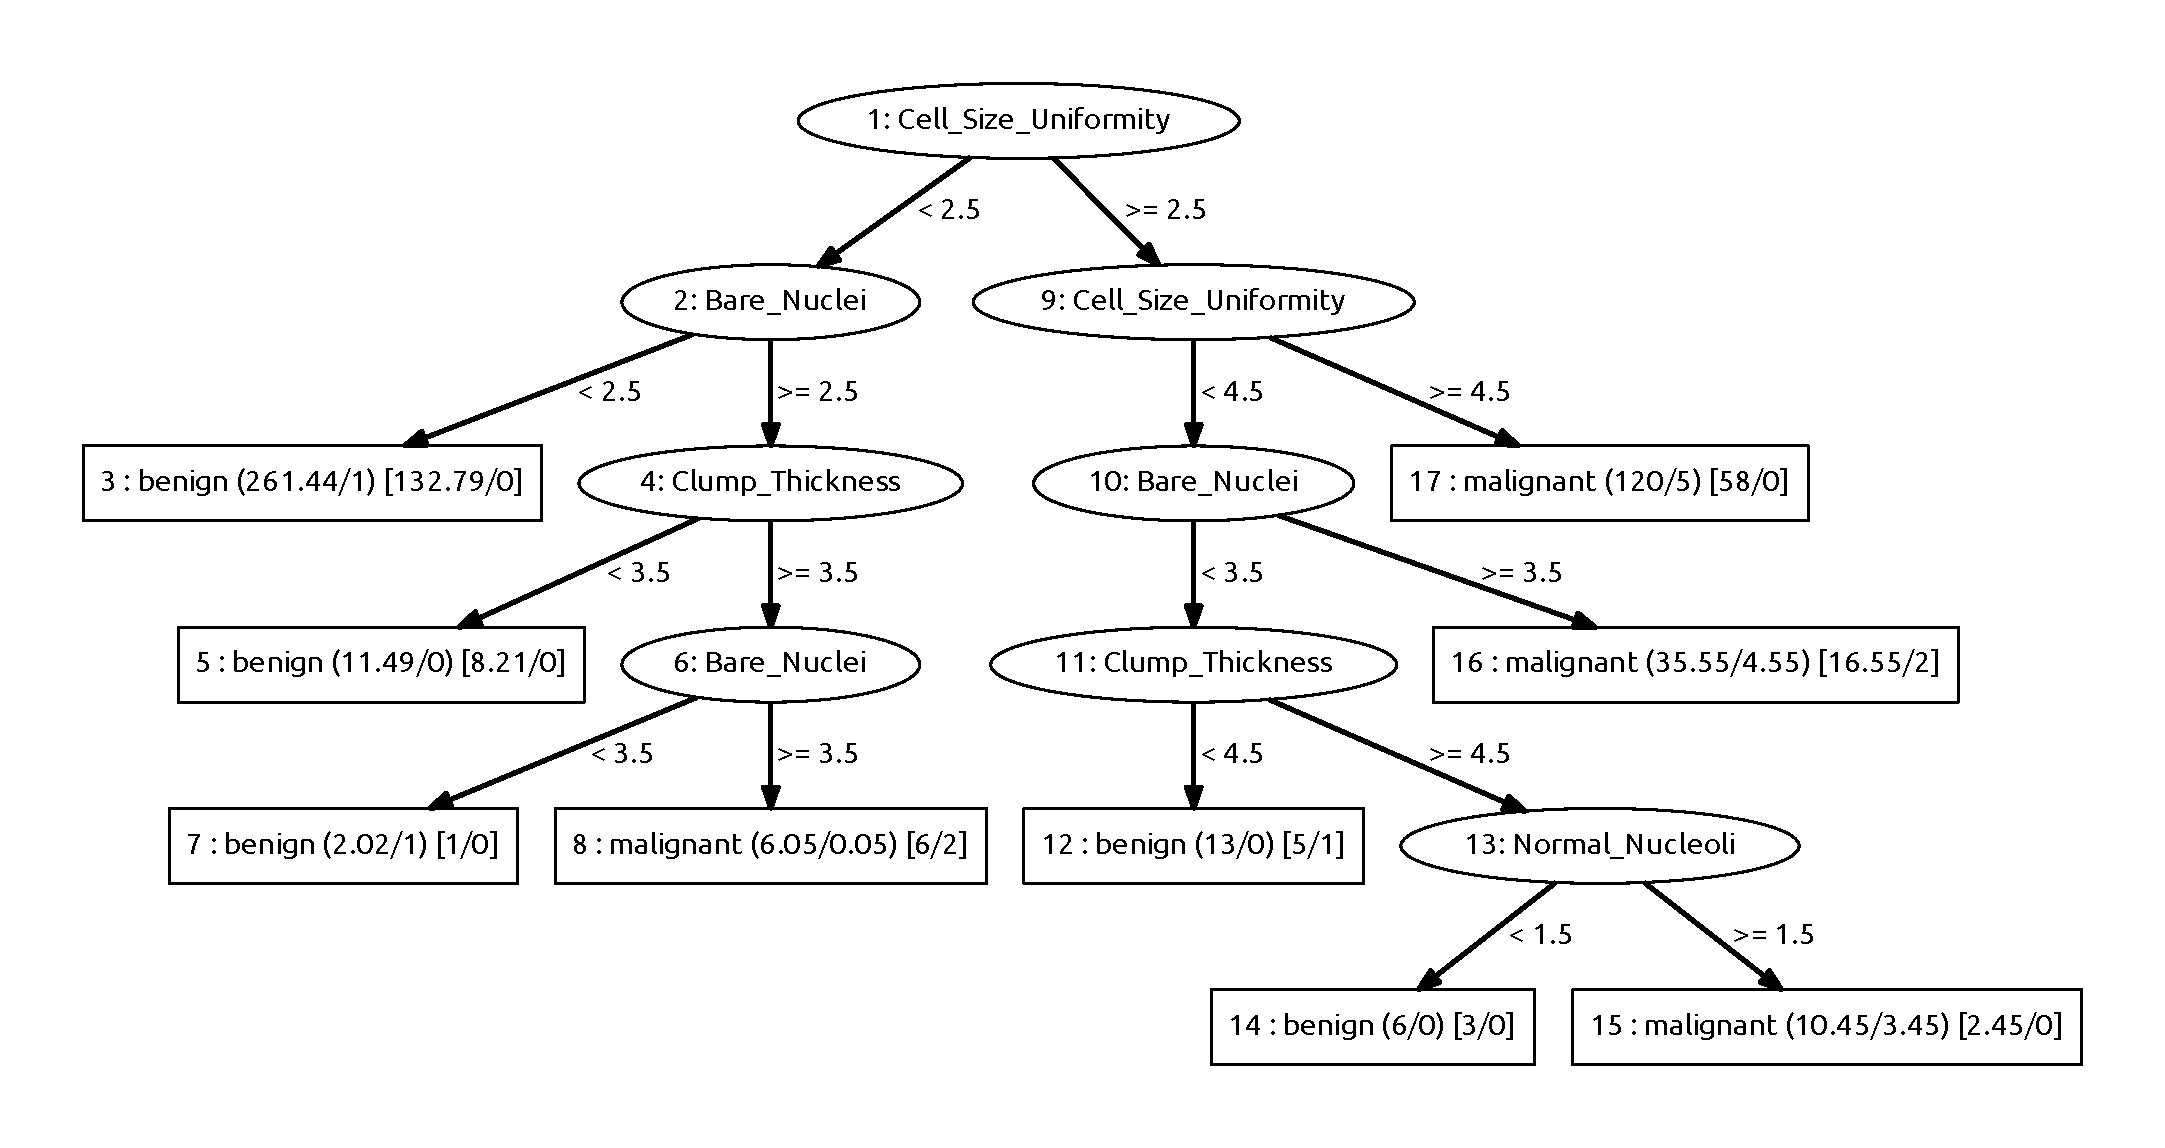
\includegraphics[width=1.55\textwidth]{results/reptree/wisconsin_breast_cancer.pdf}}
	\caption{Modello di REPTree}
\end{figure}

\begin{mdframed}[frametitle=Esecuzione JRip]
	\footnotesize\verbatiminput{results/jrip/wisconsin_breast_cancer.jrip}
\end{mdframed}


\noindent
\normalsize Regole:
\footnotesize\input{results/jrip/wisconsin_breast_cancer.list.rules}